\chapter[Capítulo 5. Conclusiones y Trabajo Futuro]{Conclusiones y Trabajo Futuro}
\section{Conclusión}
La aparición de los protocolos de buses de campo industriales ha potenciado en gran medida una importante mejora en los procesos de producción justificado principalmente en la reducción de costos y una mejora de la eficiencia permitiendo una comunicación bidireccional entre un Master y varios esclavos interconectados entre sí por un único bus. Sin embargo, uno de los principales desafíos actuales de esta tecnología se centra en que aún no se existe un único estándar para la implementación de protocolos de buses de campo. En este contexto, la implementación desarrollada en el marco de este TFG se basa en una plataforma multiprotocolo que abarca dos versiones del protocolo Modbus logrando una interoperabilidad entre redes RS232/RS485 y TCP/IP, siendo esto un punto importante debido a que las nuevas tendencias en el ámbito de buses de campo prevén una fuerte penetración de Ethernet como nivel físico de varias propuestas de buses de campo.

Otro aspecto destacable de este TFG es la versatatilidad  del \textit{software}, el mismo puede ser utilizado para desarrollar una gran cantidad de proyectos de implementación del protocolo Modbus, debido en gran medida a su arquitectura modular y a su filosofía de programación orientada a objetos logrando de esta manera un código reutilizable. El fragmento de código encargado de la implementación del protocolo fué escrito enteramente en ANSI C, pudiendo ser compilado con cualquier IDE  de C/C++; de esta manera sólo es necesario instanciar las clases que desarrollan el protocolo Modbus dentro de las clases que implementan alguna aplicación específica.

 
Finalmente es de desatacar la eficiencia lograda por plataforma diseñada cuantificada a partir de ensayos experimentales tomando como parámetro de rendimiento el porcentaje de tramas pérdidas, medidas en un ambiente bajo condiciones ruidosas, que para el peor caso pudo cuantificarse en un 1.002\%.

\section{Trabajos Futuros}
El TFG será aplicado en el proyecto desarrollado por el Departamento de Sistemas de Potencia y Control de la Facultad de Ingeniería, de manera a implementar el protocolo de comunicación entre los diferentes dispositivos que conforman la bancada experimental. El proyecto consiste en implementar un sistema de generación de energía alternativa mediante la utilización de un generador de 6 fases. El esquema del sistema  puede apreciarse en la Figura \ref{conacyt}.


\begin{figure}[h]
	\centering
		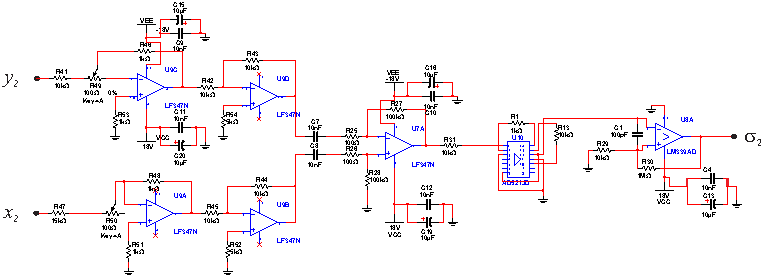
\includegraphics[height=110mm, width = 135mm]{./imagenes/plataforma08.pdf}
	\caption{Esquema del sistema de generación de energía alternativa. Fuente: Elaboración propia.}
	\label{conacyt}
\end{figure}

El \textit{software} de emulación de la turbina estará instalado en una PC que realizará el control del sistema, denominada en el gráfico como "`PC controladora del sistema"' . Este \textit{software} presisa de algunos parámetros climáticos que le serán provehidos en tiempo real, para ello es necesario tener acceso a una consola donde se almacenan los datos medidos por la estación climática \textit{Vantage Vue} de firma  \textit{Davis Instruments} que se encuentra instalada en el local del CITEC. La consola de la estación climática está conectada vía USB a otra PC desde donde varias aplicaciones extraen los datos sobre las variables climáticas, en dicha PC corre un sistema operativo Linux de la distribución Debian 6.1, la misma se encuentra rotulada en el gráfico como "`PC colectora de datos"'. Por tanto, el \textit{software} de emulacion debe comunicarse con la PC a la que está conectada la consola de manera a extraer datos de la misma.

Con el fin de extraer los datos almacenados en la consola se ha desarrollado un \textit{software} que realiza la lectura de datos cada cierto tiempo, dicho tiempo es establecido por defecto a un valor igual a 1 minuto. Los datos leídos son almacenandos en un archivo con un formato propio de la aplicación. La aplicación que realiza el almacenamiento de datos actúa como un servidor Modbus TCP, de modo que espera las solicitudes entrantes a través de la red TCP/IP, dichas solicitudes provienen desde un cliente que solicita el envío de los últimos datos climáticos almacenados, la aplicación mencionada recibe el nombre de "`Servidor Vantage-Modbus TCP"'.

Dentro del esquema de la plataforma, el cliente Modbus que se conecta al Servidor \textit{Vantage} es el \textit{software} de emulación de la turbina eólica. El \textit{software} de emulación se comporta como un cliente Modbus TCP y se conecta a la consola de almacenamiento de datos mediante la red TCP/IP, y por otro lado el \textit{software} de emulación se conecta vía Modbus RTU a un inversor de frecuencia CFW09 de la firma WEG. El \textit{software} de emulación envía al inversor de frecuencia la velocidad de referencia óptima con la cual el sistema es capaz de extraer la máxima potencia eólica del viento, dicho parámetro depende de varios factores como ser el radio de la turbina, el ángulo de ataque de las aspas y la velocidad del viento, siendo este último proveído por la estación climática \textit{Vantage Vue}.

El \textit{software} de emulación es capaz además de enviar la velocidad de referencia al inversor obtener del mismo parámetros de funcionamiento como ser la velocidad de rotación del motor trifásico, la corriente de los devanados entre otros. Por tanto dentro de la aplicación mencionada puede implementarse sistemas de monitoreo y control montado sobre un red Modbus híbrida RTU - TCP/IP con la posibilidad de hacer escalable el sistema con otras   aplicaciones como ser acceso y monitoreo mediante páginas WEB o acceso inalámbrico al sistema mediante la utilización de \textit{router} inalámbricos.


Se observa además en el esquema la interconexión del motor trifásico al generador de seis fases, mediante dicha interconexión se emula la velocidad de rotación que tendría una turbina  conectada al generador, por ende el motor trifásico gira con la misma velocidad que lo haría la turbina. El sistema de generación de seis fases es controlado mediante dos inversores de frecuencia trifásicos SKS35F de la firma \textit{Semikron}, las señales de mando y las lecturas de datos de dichos inversores pasan a travéz de un circuito acondicionador de señales diseñado para interconectar los inversores con el DSP MSK28335 de la firma \textit{Technosoft}, el cual implementa los algoritmos de control del generador de seis fases. La conexión entre la PC de control del sistema y el DSP se realiza mediante una interfaz RS232.